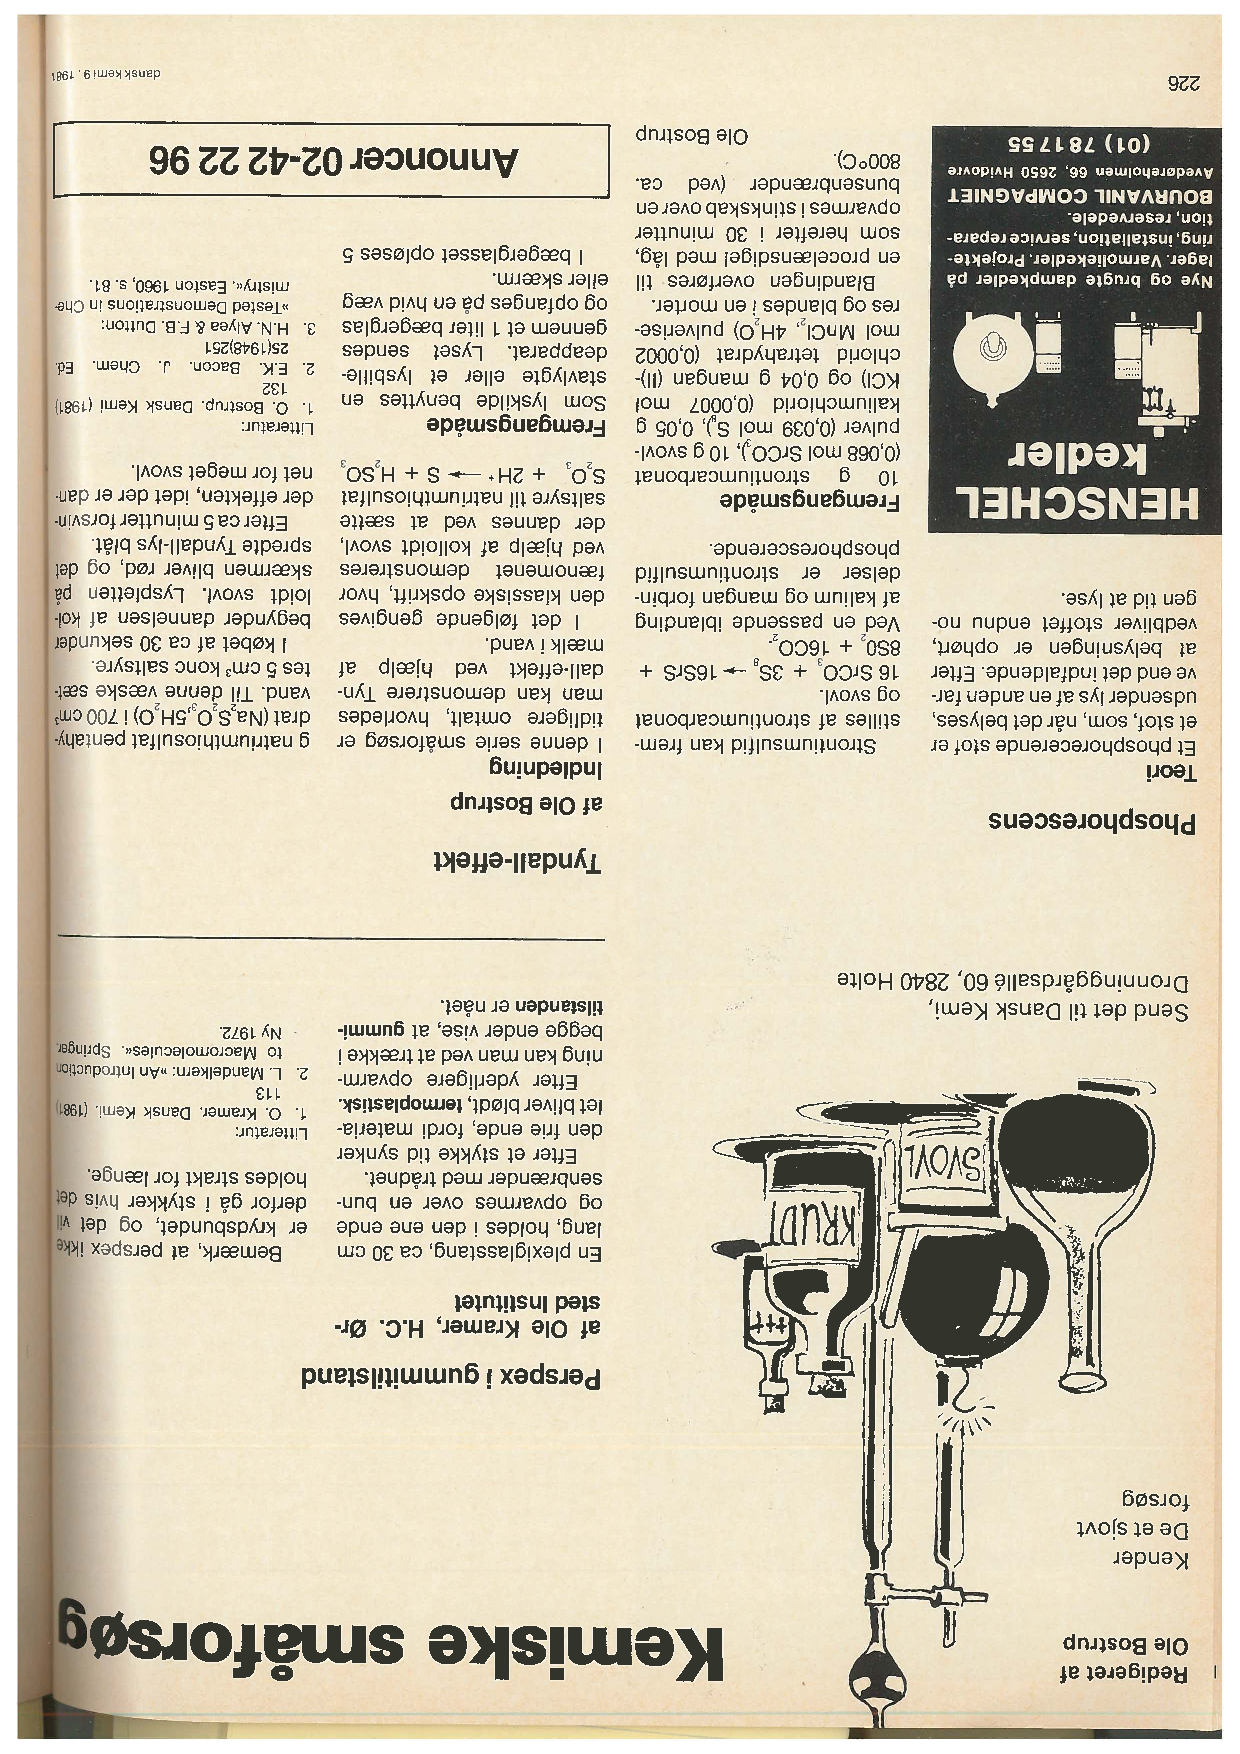
\includepdf[pages=-]{pdfs/1981-62-9-226.pdf}


\emne{Perspex i gummitilstand}
\danskkemi{Dansk Kemi 62, 3, 1981, p. 70}
\forfatter{Ole Kramer, H.C. Ørsted Institutet}

En plexiglasstang, ca 30 cm lang, holdes i den ene ende
og opvarmes over en bunsenbrænder med trådnet.
Efter et stykke tid synker den frie ende, fordi
materialet bliver blødt, \bf{termoplastiks}
Efter yderligere opvarmning kan man ved at trække i begge
ender vise, at \bf{gummitilstanden} er nået.

Bemærk at perspex ikke er krydsbundet, og det vil derfor
gå i stykker hvis det holdes strakt for længe.

Litteratur:
1. O. Kramer. Dansk Kemi, (1981) 113
2. L. Mandelkern: "An Introduction to Macromolecules".
Springer, Ny 1972.
